%\documentclass[preprint,tightenlines,showpacs,showkeys,floatfix,
%nofootinbib,superscriptaddress,fleqn]{revtex4} 
\documentclass[tightenlines,floatfix,nofootinbib,superscriptaddress,fleqn]{revtex4-2} 
%\documentclass[aps,epsfig,tightlines,fleqn]{revtex4}
\usepackage{kotex}
\usepackage[HWP]{dhucs-interword}
\usepackage[dvips]{color}
\usepackage{graphicx}
\usepackage{bm}
%\usepackage{fancyhdr}
%\usepackage{dcolumn}
\usepackage{defcolor}
\usepackage{amsmath}
\usepackage{amsfonts}
\usepackage{amssymb}
\usepackage{amscd}
\usepackage{amsthm}
\usepackage[utf8]{inputenc}
%\usepackage{tikz}
\usepackage{circuitikz}

%\pagestyle{fancy}

\begin{document}

\title{\Large 2022년 2학기 물리학 II}
\author{김현철\footnote{Office: 5S-436D (면담시간 매주
    수요일-16:15$\sim$19:00)}} 
\email{hchkim@inha.ac.kr}
\affiliation{Hadron Theory Group, Department of Physics,
  Inha  University, Incheon 22212, Republic of Korea }
\date{Autumn Semester, 2022}

\maketitle

{\color{red} {\bf Due date:} 2022년 9월 19일  15:30-16:15 }
\vspace{1.cm}

\section*{\large Quiz 6}
\noindent {\bf 문제 1 [20pt].}
그림~\ref{fig:1}처럼 평행판 축전기 한 판의 변의 길이는 각각 $10$
cm이고, 판 사이의 거리는 $d=4.0$ mm이다. 이 축전기에 들어있는 유전
물질의 유전상수는 $\kappa=2.0$이다. 
\begin{figure}[htp]
  \centering
  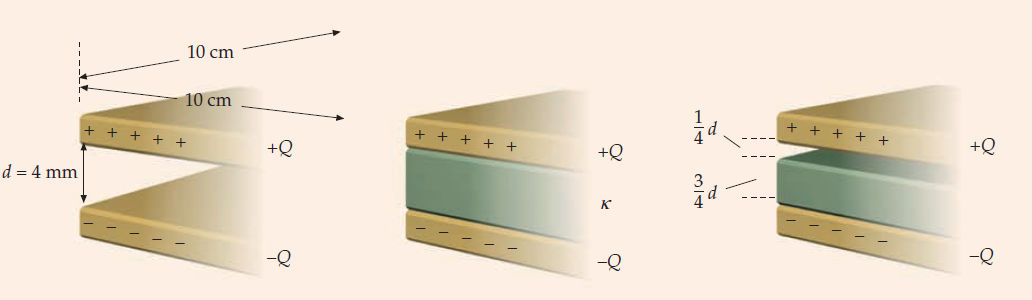
\includegraphics[scale=0.6]{qfig6-20220919-2.png}
  \caption{\textbf{문제 1}}
  \label{fig:1}
\end{figure}
\begin{itemize}
\item[(가)] 우선 평행판 축전기의 전기용량을 구하여라. 
\item[(나)] 유전물질이 들어있지 않을 때 전기용량은 얼마인가?  
\item[(다)] 만약에 양 판 사이에 유전물질이 가득 차 있다면, 이 축전기의
  전기용량은 얼마인가? 
\item[(라)] 이 두 판 사이에 크기가 $10\,\mathrm{cm}\times
  10\,\mathrm{cm}\times 3.0\,\mathrm{mm}$인 유전물질을 넣었다. 이
  축전기의 전기용량은 얼마인가? 
\end{itemize}
여기서 $\epsilon_0=8.85$ pF/m이다. 

\vspace{1.cm}
\noindent {\bf 풀이 : }
\begin{itemize}
  \item[(가)] 평행판 축전기의 전기용량은 평행판 사이 전위차로 구할 수 있다. 우선 
  크기가 같고 부호가 반대인 두 도체 사이에 $V$ 만큼의 전위차가 존재한다고 가정하자.
  이 때 전위차 $V$와 도체가 가진 전하량 $Q$는 비례하는 관계에 있다. 즉,
   \begin{align}\label{eq:1-1}
    Q = CV
   \end{align}
   이고 $C$는 앞으로 전기용량이라 부르게 될 비례상수이다. 이제 두 도체가 평행판의
   형태로 서로에 대해 평행하게 배열되어 있다고 하자. 두 평행판 사이의 거리는 $d$이고
   평행판의 면적은 $A$로 서로 같다. 평행판에 의해 평행판 사이에 생성되는 전기장 $E$의 크기는
   \begin{align}\label{eq:1-1-1}
    E = \frac{\sigma}{\epsilon_0} = \frac{Q}{\epsilon_0 A}
   \end{align}
   와 같다. $\sigma$는 면전하밀도로 평행판이 가진 전하량 $Q$를 평행판의 면적 $A$로 나눈 
   값이다. 평행판 사이가 진공이라 가정하여 진공 유전율 $\epsilon_0$에 반비례한다.
   평행판 사이 전기장 $E$도 알고 거리 $d$도 알고 있으니 평행판 사이 전위차 $V$를 구할 수 있다.
   전기장 $E$가 평행판 사이에서는 일정하므로 전위차 $V$는 전기장 $E$와 거리 $d$의 곱과 같다.
   \begin{align}
    V = -\int_d^0 \vec{E}\cdot d\vec{s} = E\int_0^d\,ds=Ed.
   \end{align}
   여기에 식~\eqref{eq:1-1-1}를 대입하여 평행판 사이 전위차 $V$를 얻을 수 있다.
   \begin{align}
    V = Ed = \frac{Q}{\epsilon_0 A}d.
   \end{align}
   이를 다시 식~\eqref{eq:1-1}에 대입하면
   \begin{align}\label{eq:1-1-2}
    Q = C\frac{Q}{\epsilon_0 A}d
   \end{align}
   를 얻는다. 우리가 구하고자 하는 것은 전기용량 $C$이므로 식~\eqref{eq:1-1-2}를 전기용량 
   $C$에 대해 정리하여
   \begin{align}\label{eq:1-1-3}
    C = \epsilon_0\frac{A}{d}
   \end{align}
   평행판 축전기의 전기용량 $C$를 얻었다.
  \item[(나)]식~\eqref{eq:1-1-3}으로부터, 면적이 $A$, 판 사이 거리 $d$이고 판 사이가 
  진공인 평행판 축전기의 전기용량 $C$는 다음과 같다.
  \begin{align}
    C = \epsilon_0\frac{A}{d}.
  \end{align}
  $A=(10~\mathrm{cm})^2=1.0\times 10^{-2}~\mathrm{m^2}$, 
  $d = 4.0~\mathrm{mm}=4.0 \times 10^{-3}~\mathrm{m}$이고 $\epsilon_0=8.85$ pF/m이므로
  평행판 축전기의 전기용량 $C$는
  \begin{align}
    C = (8.85~\mathrm{pF/m})\frac{1.0\times 10^{-2}~\mathrm{m^2}}
    {4.0 \times 10^{-3}~\mathrm{m}}
    =22~\mathrm{pF}
  \end{align}
  이다.
  \item[(다)] 유전체의 유전상수는 유전체의 유전율과 진공의 유전율의 비로 주어진다. 즉,
  \begin{align}
    \epsilon = \kappa\epsilon_0
  \end{align}
  이다. $\epsilon$는 유전체의 유전상수이다. 이 식으로부터 평행판 축전기의 사이에 유전체가
  차있는 경우와 진공인 경우의 유전상수 비를 구할 수 있다. 진공인 경우의 유전상수를 $C_0$,
  유전체가 차있는 경우의 유전상수를 $C$라고 한다면 $C/C_0$는
  \begin{align}
    \frac{C}{C_0}=\left(\epsilon\frac{A}{d}\right)
    \left(\epsilon_0\frac{A}{d}\right)^{-1}
    =\frac{\epsilon}{\epsilon_0}=\kappa
  \end{align}
  유전체의 유전상수와 같다. 따라서 유전체가 가득 찬 평행판 축전기의 전기용량 $C$는
  \begin{align}
    C = \kappa C_0 = (2.0)(22~\mathrm{pF})=44~\mathrm{pF}
  \end{align}
  $44~\mathrm{pF}$이다.
  \item[(라)]
   
  %유전체가 평행판 사이를 길이 $\frac{3}{4}d$ 만큼만 채운 축전기는
  %평행판 사이 거리가 $\frac{1}{4}d$이고 평행판 사이가 진공인 평행판 축전기 $A$와
  %평행판 사이 거리가 $\frac{3}{4}d$이고 유전체로 가득 채워진 평행판 축전기 $B$의 직렬 연결로
  %생각할 수 있다. 
  %직렬로 연결된 축전기들은 각각에 축전되는 전하량이 같으므로 축전기 $A$, 축전기 $B$와
  %두 축전기가 합쳐진 원래의 축전기 $C$에 축전되는 전하량은 $Q$로 같다. 따라서,
  %\begin{align}
  %  Q = C_1V_1=C_2V_2=C_3V_3
  %\end{align}
  %거리가 $\frac{1}{4}d$인 평행판 축전기에 걸리는 전압을 $V_1$, 
  %거리가 $\frac{3}{4}d$이고 유전체로 가득 채워진 평행판 축전기에 걸리는 전압을 $V_2$라 하자. 

\end{itemize}



\vspace{1.cm}

\noindent {\bf 문제 2 [20pt].} 100 W 전구를 120 V 전원에 꽂았다.
\begin{itemize}
\item[(가)] 전구를 계속해서 켜두려면, 31일 동안의 비용은 얼마인가?
  전기에너지의 가격은 60 원 / $\mathrm{kW\cdot h}$라고 가정한다.
\item[(나)] 전구의 저항은 얼마인가?
\item[(다)] 전구에 흐르는 전류는 얼마인가? 
\end{itemize}
\noindent {\bf 풀이 : }
\begin{itemize}
  \item[(가)] 100 W 전구를 31일 동안 켜두었을 때 소모되는 전기 에너지 $W$는
  \begin{align}
    W = (100~\mathrm{W})(31~\text{일}) = (100~\mathrm{W})(31~\text{일})
    \left(\frac{24~\text{h}}{1~\text{일}}\right)
    =74\,000~\mathrm{W\cdot h}=74~\mathrm{kW\cdot h}
  \end{align}
 이다. 따라서 31일 동안 켜두었을 때 지불해야할 비용 $A$는
 \begin{align}
  A = (60~\text{원}/\mathrm{kW\cdot h})(74~\mathrm{kW\cdot h})
  =4440~\text{원}
 \end{align}
 4400원이다.
  \item[(나)] 줄의 법칙에 의해 전구의 일률 $P = $100 W는 전구에 걸리는 전압 $V=120$ V와
  전구의 저항 $R$에 대해 다음의 관계에 있다.
  \begin{align}
    P = \frac{V^2}{R}.
  \end{align}
  따라서 전구의 저항 $R$은
  \begin{align}
    R = \frac{V^2}{P} = \frac{(120~\mathrm{V})^2}{100~\mathrm{W}}
    =144~\mathrm{\Omega}
  \end{align}
  144$~\mathrm{\Omega}$이다.
  \item[(다)] 전구에 흐르는 전류 $I$는 옴의 법칙을 통해 구할 수 있다. 옴의 법칙으로부터
  전구에 흐르는 전류 $I$는
  \begin{align}
    I=\frac{V}{R} = \frac{120~\mathrm{V}}{144~\mathrm{\Omega}}
    =0.83~\mathrm{A}
  \end{align}
  0.83 A이다.
  
\end{itemize}


\newpage


\noindent {\bf 문제 3 [20pt].} 
\begin{figure}[htp]
  \centering
  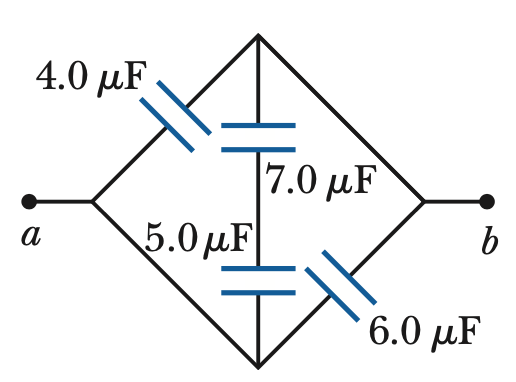
\includegraphics[scale=0.5]{qfig7-1.png}
  \caption{\textbf{문제 3}}
  \label{fig:3}
\end{figure}
그림~\ref{fig:3}에 주어진 $a$와 $b$ 사이에 연결되어 있는 이 축전기들의
등가 전기용량을 구하여라.  

\noindent {\bf 풀이 : }

\begin{figure}[htbp]
  \centering
  \scalebox{.8}{
  \begin{circuitikz}
    [declare function = {d = 2;}]
    \ctikzset{label/align = straight}
  \draw     (-d,0) node[label = {$A$}](A){}
  to [C,l^= $C_1$,*-*] (0,d) node[label = {$B$}](B){}
  to        ( d,0) node[label = {$C$}](C){}
  to [C,l= $C_2$,*-*](0,-d) node[label = {below:$D$}](D){}
  to        (-d,0) 
  (B) to [C,l= $C_3$] (0,0) 
  (0,0) to [C,l_= $C_4$] (D)
  (A) to ++(-1,0) node[label = {$a$}](a){}
  (C) to ++(1,0) node[label = {$b$}](b){}
  ;
\end{circuitikz}
\begin{circuitikz}
  [declare function = {d = 2;}]
  \ctikzset{label/align = straight}
\draw     (-d,0) node[label = {$A$}](A){}
to [C,l^= $C_1$,*-*] (0,d) node[label = {$B$}](B){}
to        ( d,0) node[label = {$C$}](C){}
to [C,l= $C_2$,*-*](0,-d) node[label = {below:$D$}](D){}
to        (-d,0) 
(B) to [C,l= $C_5$] (D)
(A) to ++(-1,0) node[label = {$a$}](a){}
(C) to ++(1,0) node[label = {$b$}](b){}
;
\end{circuitikz}
  }
  \caption{$C_3$, $C_4$의 합성}
  \label{fig:3-1}
\end{figure}

\noindent 먼저 각 전선들이 만나는 마디들을 FIG.~\ref{fig:3-1}와 같이 $A,\,B,\,C,\,D$라 하고 각
축전기들의 전기용량을 $C_1,\,C_2,\,C_3,\,C_4$라고 하자. 직렬로 연결된 축전기의 전기용량
$C_3,\,C_4$를 합성한 전기용량 $C_5$는 다음과 같이 구할 수 있다(FIG.~\ref{fig:3-1}).
\begin{align}
  \frac{1}{C_5} = \frac{1}{C_3}+\frac{1}{C_4} \Longrightarrow
  C_5 = \frac{C_3C_4}{C_3+C_4}.
\end{align}

\begin{figure}[htbp]
  \centering
  \scalebox{.8}{
  \begin{circuitikz}
    [declare function = {d = 2;}]
    \ctikzset{label/align = straight}
  \draw (-d,d) node[label = {$A$}](A){}
  to [C,l^= $C_1$,*-*] (d,d) node[label = {$B$}](B){}
  to (d,0) node[label = {right:$B'$}](B'){}
  to (d,-d) node[label = {below:$C$}](C){}
  to [C,l_= $C_2$,*-*] (-d,-d) node[label = {below:$D$}](D){}
  to (-d,0) node[label = {left:$D'$}](D'){}
  to (A)
  (D') [C,l= $C_5$,*-*] to (B')
  (A) -- ++(-1,0) node[label = {above:$a$}](a){}
  (C) -- ++(1,0) node[label = {above:$b$}](b){}
  ;
\end{circuitikz}
  }
  \caption{fig~\ref{fig:3-1}의 병렬화}
  \label{fig:3-2}
\end{figure}

이제 축전기 $C_5$가 연결된 마디 $B$와 $D$를 이동시켜 축전기 $C_5$ 새로운 마디 $B'$와 $D'$에
연결되어 있다고 생각하자(FIG.~\ref{fig:3-2}). 마디는 같은 도선 내에서 움직인 것이므로 
마디를 이동시키기 전의 회로와 후의 회로는 동일하다. 이 회로는 축전기 $C_1$, $C_5$, $C_2$가
병렬로 연결된 회로이므로 세 축전기의 합성 전기용량 $C_{tot}$는
\begin{align}
  C_{tot} = C_1 + C_5 + C_2 = C_1 + C_2 + \frac{C_3C_4}{C_3+C_4}
\end{align}
이다. 각각의 전기용량들은 $C_1= 4.0~\mathrm{\mu F},\,C_2= 6.0~\mathrm{\mu F},\,
C_3= 7.0~\mathrm{\mu F},\,C_4= 6.0~\mathrm{\mu F}$로 주어졌으므로 $C_{tot}$의 값은 다음과
같이 계산하여 얻을 수 있다.
\begin{align}
  \begin{split}
    C_{tot} &= 4.0~\mathrm{\mu F}+6.0~\mathrm{\mu F}
    +\frac{(7.0~\mathrm{\mu F})(6.0~\mathrm{\mu F})}
    {(7.0~\mathrm{\mu F})+(6.0~\mathrm{\mu F})} \\
    &= 13~\mathrm{\mu F}.
  \end{split}
\end{align}
따라서 회로의 등가 전기용량 $C_{tot}$는 $13~\mathrm{\mu F}$이다.
\vspace{1.cm}

\noindent {\bf 문제 4 [20pt].} 
가벼운 전기자동차가 있다. 이 차는 12.0 V의 배터리를 직렬로 연결해서
힘을 얻는다. 이 각각의 배터리 내부 저항은 무시할 수 있다. 각각의
배터리는 다시 충전하기 전까지 $160\,\mathrm{A\cdot h}$의 전하를
자동차에 전달한다. 이 자동차가 80.0 km/h의 속력으로 갈 때 이 자동차가
맏는 공기 저항과 구름마찰력(rolling friction)은 1.20 kN이다. 
\begin{itemize}
\item[(가)] 만약에 자동차가 80.0 km/h로 가고 있을 때 전기 모터가
  자동차에 전해주는 최소 일률은 얼마인가?
\item[(나)] 충전이 필요하기 전까지 이 직렬로 연결되어 있는 열 개의
  배터리가 전달하는 총전하는 얼마인가?(coulomb의 단위를 써서
  나타내어라.) 
\item[(다)] 재충전이 필요하기 전까지 열 개의 배터리가 전달하는 총
  전기에너지는 얼마인가? 
\item[(라)] 배터리가 재충전을 필요로 하기 전까지 이 자동차는 얼마나
  멀리 갈 수 있는가?(자동차의 속력은 80.0 km/h로 일정하다.)
\item[(마)] 배터리를 충전하는 데 1 kW-h 당 100원이 든다면, 킬로미터 당
  전기료는 얼마가 필요한가? 
\end{itemize}

\vspace{1.cm}
\noindent {\bf 풀이 : }
\vspace{1.cm}

\end{document}